% Created by tikzDevice version 0.10.1 on 2017-11-27 12:50:34
% !TEX encoding = UTF-8 Unicode
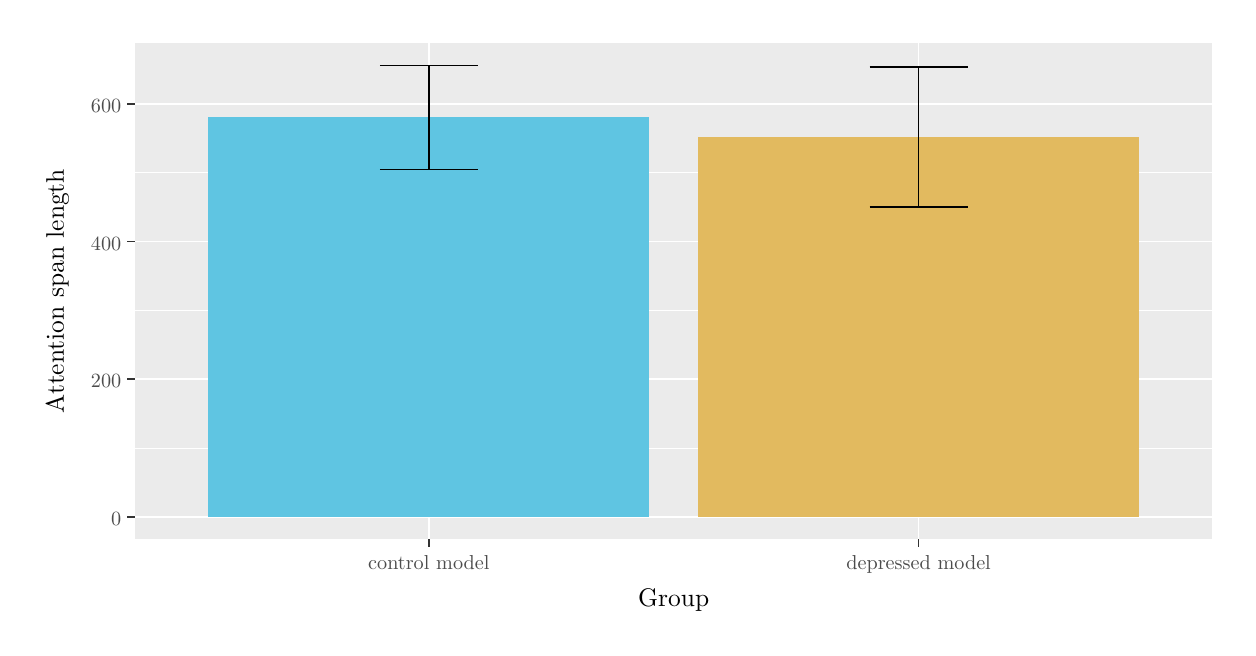
\begin{tikzpicture}[x=1pt,y=1pt]
\definecolor{fillColor}{RGB}{255,255,255}
\path[use as bounding box,fill=fillColor,fill opacity=0.00] (0,0) rectangle (433.62,216.81);
\begin{scope}
\path[clip] (  0.00,  0.00) rectangle (433.62,216.81);
\definecolor{drawColor}{RGB}{255,255,255}
\definecolor{fillColor}{RGB}{255,255,255}

\path[draw=drawColor,line width= 0.6pt,line join=round,line cap=round,fill=fillColor] (  0.00,  0.00) rectangle (433.62,216.81);
\end{scope}
\begin{scope}
\path[clip] ( 38.78, 31.92) rectangle (428.12,211.31);
\definecolor{fillColor}{gray}{0.92}

\path[fill=fillColor] ( 38.78, 31.92) rectangle (428.12,211.31);
\definecolor{drawColor}{RGB}{255,255,255}

\path[draw=drawColor,line width= 0.3pt,line join=round] ( 38.78, 64.93) --
	(428.12, 64.93);

\path[draw=drawColor,line width= 0.3pt,line join=round] ( 38.78,114.63) --
	(428.12,114.63);

\path[draw=drawColor,line width= 0.3pt,line join=round] ( 38.78,164.34) --
	(428.12,164.34);

\path[draw=drawColor,line width= 0.6pt,line join=round] ( 38.78, 40.07) --
	(428.12, 40.07);

\path[draw=drawColor,line width= 0.6pt,line join=round] ( 38.78, 89.78) --
	(428.12, 89.78);

\path[draw=drawColor,line width= 0.6pt,line join=round] ( 38.78,139.49) --
	(428.12,139.49);

\path[draw=drawColor,line width= 0.6pt,line join=round] ( 38.78,189.19) --
	(428.12,189.19);

\path[draw=drawColor,line width= 0.6pt,line join=round] (144.96, 31.92) --
	(144.96,211.31);

\path[draw=drawColor,line width= 0.6pt,line join=round] (321.94, 31.92) --
	(321.94,211.31);
\definecolor{fillColor}{RGB}{95,197,226}

\path[fill=fillColor] ( 65.33, 40.07) rectangle (224.60,184.36);
\definecolor{fillColor}{RGB}{226,186,95}

\path[fill=fillColor] (242.30, 40.07) rectangle (401.57,177.28);
\definecolor{drawColor}{RGB}{0,0,0}

\path[draw=drawColor,line width= 0.6pt,line join=round] (127.27,203.16) --
	(162.66,203.16);

\path[draw=drawColor,line width= 0.6pt,line join=round] (144.96,203.16) --
	(144.96,165.56);

\path[draw=drawColor,line width= 0.6pt,line join=round] (127.27,165.56) --
	(162.66,165.56);

\path[draw=drawColor,line width= 0.6pt,line join=round] (304.24,202.49) --
	(339.63,202.49);

\path[draw=drawColor,line width= 0.6pt,line join=round] (321.94,202.49) --
	(321.94,152.08);

\path[draw=drawColor,line width= 0.6pt,line join=round] (304.24,152.08) --
	(339.63,152.08);
\end{scope}
\begin{scope}
\path[clip] (  0.00,  0.00) rectangle (433.62,216.81);
\definecolor{drawColor}{gray}{0.30}

\node[text=drawColor,anchor=base east,inner sep=0pt, outer sep=0pt, scale=  0.73] at ( 33.83, 37.04) {0};

\node[text=drawColor,anchor=base east,inner sep=0pt, outer sep=0pt, scale=  0.73] at ( 33.83, 86.75) {200};

\node[text=drawColor,anchor=base east,inner sep=0pt, outer sep=0pt, scale=  0.73] at ( 33.83,136.46) {400};

\node[text=drawColor,anchor=base east,inner sep=0pt, outer sep=0pt, scale=  0.73] at ( 33.83,186.16) {600};
\end{scope}
\begin{scope}
\path[clip] (  0.00,  0.00) rectangle (433.62,216.81);
\definecolor{drawColor}{gray}{0.20}

\path[draw=drawColor,line width= 0.6pt,line join=round] ( 36.03, 40.07) --
	( 38.78, 40.07);

\path[draw=drawColor,line width= 0.6pt,line join=round] ( 36.03, 89.78) --
	( 38.78, 89.78);

\path[draw=drawColor,line width= 0.6pt,line join=round] ( 36.03,139.49) --
	( 38.78,139.49);

\path[draw=drawColor,line width= 0.6pt,line join=round] ( 36.03,189.19) --
	( 38.78,189.19);
\end{scope}
\begin{scope}
\path[clip] (  0.00,  0.00) rectangle (433.62,216.81);
\definecolor{drawColor}{gray}{0.20}

\path[draw=drawColor,line width= 0.6pt,line join=round] (144.96, 29.17) --
	(144.96, 31.92);

\path[draw=drawColor,line width= 0.6pt,line join=round] (321.94, 29.17) --
	(321.94, 31.92);
\end{scope}
\begin{scope}
\path[clip] (  0.00,  0.00) rectangle (433.62,216.81);
\definecolor{drawColor}{gray}{0.30}

\node[text=drawColor,anchor=base,inner sep=0pt, outer sep=0pt, scale=  0.73] at (144.96, 20.91) {control model};

\node[text=drawColor,anchor=base,inner sep=0pt, outer sep=0pt, scale=  0.73] at (321.94, 20.91) {depressed model};
\end{scope}
\begin{scope}
\path[clip] (  0.00,  0.00) rectangle (433.62,216.81);
\definecolor{drawColor}{RGB}{0,0,0}

\node[text=drawColor,anchor=base,inner sep=0pt, outer sep=0pt, scale=  0.92] at (233.45,  7.83) {Group};
\end{scope}
\begin{scope}
\path[clip] (  0.00,  0.00) rectangle (433.62,216.81);
\definecolor{drawColor}{RGB}{0,0,0}

\node[text=drawColor,rotate= 90.00,anchor=base,inner sep=0pt, outer sep=0pt, scale=  0.92] at ( 13.08,121.61) {Attention span length};
\end{scope}
\end{tikzpicture}
